\documentclass[../proyecto.tex]{memoir}

\begin{document}

\chapter{Análisis}

Las estimaciones de los métodos Monte Carlo dependen en gran medida de la anchura del intervalo de confianza $[\mu+3\sigma, \mu-3\sigma]$. Dicha anchura se reduce con el incremento del número de muestras aleatorias pero lo hace lentamente con el consecuente incremento de tiempo de computación. Por esta razón se crean métodos alternativos conocidos como métodos de reducción de la varianza. En esta sección introducimos uno que se adecúa a nuestro problema, que utilizaremos en las todas las ejecuciones posteriores y a continuación procedemos a estudiar el efecto de la $\alpha$-asincronicidad en la evolución de algunas configuraciones.

\section{Reducción de la varianza}

El intervalo de confianza $[\mu+3\sigma, \mu-3\sigma]$ crece a medida que la iteración se aleja de la configuración inicial, de decir, la varianza aumenta. Es posible reducirla aumentando el número de simulaciones globalmente e incrementando notablemente el tiempo de cálculo. Por tanto proponemos incrementar el número de simulaciones a medida que las iteraciones aumenten. Este incremento requiere de la adición de nuevas simulaciones en cada iteración, las cuales serán escogidas aleatoriamente de las ya existentes modificando la semilla para no obtener simulaciones duplicadas. Experimentalmente hemos observado que un valor que muestra buenos resultados sin aumentar excesivamente el tiempo de cálculo es un incremento en cada iteración de una décima parte del valor inicial de simulaciones. 

Finalmente es posible observar la reducción del intervalo de confianza que conlleva dicho incremento en la \autoref{fig:33}, dónde visualizamos la evolución del promedio de nodos ocupados en cada iteración del juego de vida. Para el contenido de esta sección no es relevante la configuración de la que se han obtenido los datos. Cada punto representa una estimación Monte Carlo junto con el intervalo de confianza $[\mu+3\sigma, \mu-3\sigma]$.

\begin{figure}[H]
	\centering
	\begin{subfigure}[b]{0.9\textwidth} 
		\centering
    	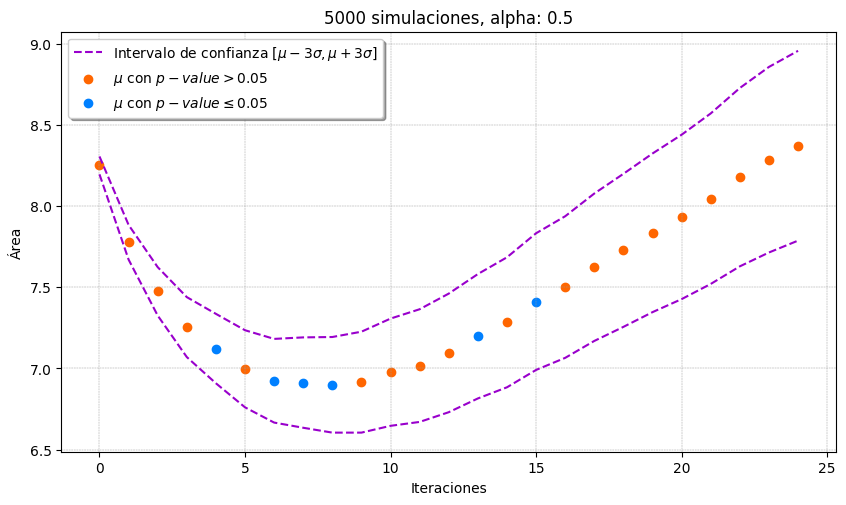
\includegraphics[width=\textwidth]{./images/iteracion_without_inc.png}
    	\caption{Ejecución sin incremento del valor inicial de simulaciones cada iteración.}
    	\label{fig:3-1}
    \end{subfigure}
    \\
	\begin{subfigure}[b]{0.9\textwidth} 
        \centering
        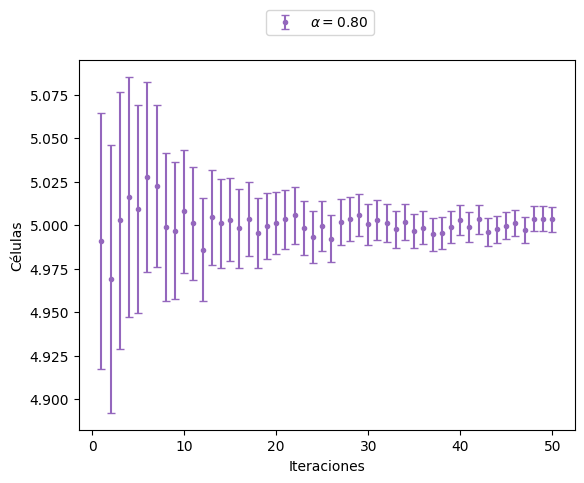
\includegraphics[width=\textwidth]{./images/iteracion_inc.png}
        \caption{Ejecución con incremento del 10\% del valor inicial de simulaciones en cada iteración.}
        \label{fig:3-2}
    \end{subfigure}
    \caption{Aplicación del método de reducción de varianza.}
    \label{fig:33}
\end{figure} 

\section{$\alpha$-asincronismo en la evolución de las configuraciones iniciales}

En esta sección vamos a estudiar el impacto de la $\alpha$-asíncronicidad. Las configuraciones iniciales son las escogidas en la sección \ref{seleccion}. Las ejecuciones son de 50 iteraciones con los valores de $\alpha$: 0.15, 0.3, 0.45, 0.6, 0.75 y 0.9. Cada iteración simulada 5000 veces aplicando el método de reducción de la varianza descrito en la sección anterior. Como resultado hemos obtenido los valores medios de las variables expuestas en la sección \ref{vars} junto con sus correspondientes intervalos de confianza para cada iteración.

\subsection{\textit{Osciladores} de periodo 2} \label{osci2}

Comentamos los efectos de la variación de la $\alpha$-asincronicidad sobre la configuración inicial \textit{blinker}. Como se observa en la \autoref{fig:blinker_evo}, cuando no existe perturbación en el intercambio de información entre nodos ocupados, el calor en cada iteración es 4, es decir, 2 nodos se liberan y 2 nodos se ocupan iteración, ocupa un área de 3 \textit{nodos}$^2$ y está conformada por un solo clúster. En primer lugar, podemos observar en la \autoref{fig:4-1} que los valores de $\alpha$ se aproximan inferiormente a $0.5$, imprimen un cambio de crecimiento en el área media. Mientras que para $\alpha=0.15$, el promedio de área a partir la vigésima iteración decrece ligeramente, para $\alpha=0.3$ el decrecimiento prácticamente desaparece, adquiriendo un valor constante y a partir de $\alpha=0.45$ comienza una acusada tendencia de crecimiento. Esta tendencia se incrementa cuando $\alpha$ se aproxima a la unidad. En particular para $\alpha=0.60$ el crecimiento a partir de la décima iteración mantiene su pendiente, hecho que no se repite para $\alpha=0.75$, donde en la vigésima iteración cambia ligeramente la pendiente y finalmente en la décimo quinta iteración de $\alpha=0.9$, el cambio de pendiente es más notable y desacelera marcadamente el crecimiento del área media. A la vez que estos fenómenos ocurren, la iteración a partir de la cual se produce el crecimiento del área media, decrece. Ésto es algo más visible en los valores de $\alpha$ superiores a $0.5$.

Si observamos la \autoref{fig:4-2}, contemplamos un comportamiento similar al descrito anteriormente, por tanto resulta interesante explorar el valor medio de densidad que relaciona la variación conjunta de ambas variables. 

\begin{figure}[H]
	\centering
	\begin{subfigure}[b]{0.9\textwidth} 
		\centering
    	\includegraphics[width=\textwidth]{./images/data/blinker/{Area_multiple_alpha}.png}
    	\caption{}
    	\label{fig:4-1}
    \end{subfigure}
    \\
	\begin{subfigure}[b]{0.9\textwidth} 
        \centering
        \includegraphics[width=\textwidth]{./images/data/blinker/{Celulas_multiple_alpha}.png}
        \caption{}
        \label{fig:4-2}
    \end{subfigure}
	\\
    \caption{Variación del área y número de nodos ocupados medio en la configuración \textit{blinker} para distintos valores de $\alpha$.}
    \label{fig:44}
\end{figure} 

El fenómeno de decrecimiento del número de iteración a partir del cual se producen los cambios descritos anteriormente, se puede visualizar más claramente en la \autoref{fig:4-3}. Cuando $\alpha$ se incrementa, la iteración a partir del cual la densidad se vuelve constante decrece. Por ejemplo, en la vigésima iteración $\alpha=0.3$ el valor medio de densidad se torna constante. Otra de las cuestiones que es posible observar sobre la variación de la densidad media es que cuando $\alpha$ crece, el valor medio de densidad constante que se alcanza se hace cada vez menor. Ésto nos informa de que durante esas iteraciones el área crece en mayor medida que el número de nodos ocupados, obteniéndose valores menores de densidad.

\begin{figure}[H]
	\centering
    \includegraphics[width=0.9\textwidth]{./images/data/blinker/{Densidad_multiple_alpha}.png}
    \caption{Evolución de la densidad media de la configuración \textit{blinker} para distintos valores de $\alpha$.}
    \label{fig:4-3}
\end{figure}

La \autoref{fig:5-1} muestra la variación del calor medio para distintos valores de $\alpha$. Se pueden observar dos zonas de cambio respecto a $\alpha$, una dada por los valores de $\alpha$ menores a $0.5$ y otra por los valores superiores. La primera se caracteriza por un fuerte descenso del calor hasta el rango de iteraciones 15-20, a continuación o bien se estabiliza ($\alpha=0.45$) o bien decrece ligeramente ($\alpha=0.15,0.30$). La segunda zona decrece en mucho menor medida que la anterior, hasta el rango de iteraciones 10-15 y después para $\alpha=0.6$ crece ligeramente con una pendiente constante. A diferencia de los valores $\alpha=0.75,0.90$ que la tienen más pronunciada de la décima a la vigésima iteración y a partir de esta última, cambia frenando el desacelerando del valor medio. De hecho, el calor promedio para $\alpha=0.9$ sugiere la existencia de una asíntota vertical con un calor medio igual a 3 nodos. A diferencia de los valores medios anteriormente comentados, el crecimiento que experimenta el calor cuando es mucho menos marcado y no llega a superar los valores iniciales. 

Si consultamos la \autoref{fig:5-2} que recoge la variación del número de clústeres medio respecto de $\alpha$, observamos la diferencia principal con la \autoref{fig:5-1} es que para valores de $\alpha$ mayores o iguales a $0.45$ el promedio de clústeres decrece en aproximadamente la décima iteración a un valor cercano a $0.6$, a partir de esta iteración el comportamiento es muy similar al del calor medio. En particular, el cambio de pendiente a partir de la décima iteración se reconoce unicamente para $\alpha=0.9$, mientras que para $\alpha=0.45,0.60,0.75$ la pendiente es prácticamente constante.

\begin{figure}[H]
	\centering
	\begin{subfigure}[b]{0.9\textwidth} 
		\centering
    	\includegraphics[width=\textwidth]{./images/data/blinker/{Calor_multiple_alpha}.png}
    	\caption{}
    	\label{fig:5-1}
    \end{subfigure}
    \\
	\begin{subfigure}[b]{0.9\textwidth} 
        \centering
        \includegraphics[width=\textwidth]{./images/data/blinker/{Clusteres_multiple_alpha}.png}
        \caption{}
        \label{fig:5-2}
    \end{subfigure}
    \caption{Variación del calor y número de clústeres medio en la configuración \textit{blinker} para distintos valores de $\alpha$.}
    \label{fig:55}
\end{figure}

El otro oscilador de periodo dos que hemos estudiado, la configuración \textit{toad} (\autoref{fig:toad_evo}) formada por 6 nodos ocupados que ocupan un área de 8 \textit{nodos}$^2$ en las iteraciones pares y 16 \textit{nodos}$^2$ en las impares, muestra un comportamiento muy similar a \textit{blinker} frente a la introducción de $\alpha$-asíncronismo en su evolución. Por ejemplo, en la \autoref{fig:66} se puede apreciar como el comportamiento es profundamente similar al mostrado en la \autoref{fig:4-2}.

\begin{figure}[H]
		\centering
    	\includegraphics[width=\textwidth]{./images/data/toad/{Area_multiple_alpha}.png}
    \caption{Variación del área media en la configuración \textit{toad} para distintos valores de $\alpha$.}
    \label{fig:66}
\end{figure}

\subsection{\textit{Osciladores} de periodo 3}

\subsection{\textit{Osciladores} de periodo 4}

\subsection{\textit{Naves espaciales}}
Hasta ahora solo hemos descrito el comportamiento de \textit{osciladores}. Como se expuso en la sección \ref{spaceships}, las \textit{naves espaciales} pueden ser vistas como \textit{osciladores} que se desplazan, luego es interesante explorar si los comportamientos que hemos observado en las configuraciones iniciales anteriores se reproducen en este tipo de configuraciones iniciales. 

Comenzamos la sección estudiando la configuración inicial \textit{lightweight spaceship} (\autoref{fig:lightweightspaceship}). En la \autoref{fig:lightweightspaceship_evo} se muestran 4 iteraciones de esta configuración inicial. Se trata de una configuración de velocidad $c/2$ que se desplaza paralelamente al eje horizontal con un área constante de 20 \textit{nodos}$^2$. En las iteraciones pares tiene 9 nodos ocupados agrupados en dos clústeres con un calor de [MISSING VALUE!] nodos y en las iteraciones impares tiene 12 nodos agrupados en un solo clúster con un calor de 8 nodos.

\begin{figure}[H]
	\centering
    
\includegraphics[width=\textwidth]{./images/lightweightspaceship_evo.png}
    \caption{De derecha a izquierda, evolución síncrona de la configuración \textit{lightweightspaceship}.}
    \label{fig:lightweightspaceship_evo}
\end{figure}

Uno de los característicos efectos que produce la introducción de $\alpha$-asincronismo en esta configuración inicial es que el número de clústeres permanece constante durante en todas la ejecución (\autoref{fig:7-1}). Ésto contrasta con el hecho de que el resto de variables observadas tomen un valor diferente para cada valor de $\alpha$. Si observamos el número medio de nodos ocupados(\autoref{fig:7-2}) se observa que tras superar la décimo quinta iteración los valores medios se estabilizan y la separación vertical de dichos valores constantes es aproximadamente igual a 0.5 nodos ocupados entre valores consecutivos de $\alpha$. De esta manera el observamos que cuando el valor de $\alpha$ el promedio nodos ocupados se acerca a los 12 nodos ocupados en la iteraciones impares de esta configuración con la evolución síncrona.

Mientras que la densidad y el calor medios de esta configuración tienen un comportamiento similar al número medio de nodos ocupados se puede observar una variación diferente en el área media (\autoref{fig:7-3}). Cuando $\alpha$ se aproxima, tanto inferior como superiormente, a $0.5$ los valores medios de área se estabilizan entorno al valor 21.2 \textit{nodos}$^2$. Por otro lado cuando $\alpha$ se aproxima a 0 ó a 1, los valores medios se aproximan a 20.5 \textit{nodos}$^2$, un valor muy cercano a los 20 \textit{nodos}$^2$ de la configuración con evolución síncrona. Otra cuestión notable es que el valor de área media pertenece en el intervalo $(20.5, 21.5)$ cuando $\alpha$ varía, un intervalo de pequeña longitud. A diferencia de la longitud de los intervalos en los que se encuentran los promedios de nodos ocupados, densidad y calor, que es mayor.

\begin{figure}[H]
	\centering
	\begin{subfigure}[b]{0.9\textwidth} 
		\centering
    	\includegraphics[width=\textwidth]{./images/data/lightweightspaceship/{Clusteres_multiple_alpha}.png}
    	\caption{}
    	\label{fig:7-1}
    \end{subfigure}
    \\
	\begin{subfigure}[b]{0.9\textwidth} 
        \centering
        \includegraphics[width=\textwidth]{./images/data/lightweightspaceship/{Celulas_multiple_alpha}.png}
        \caption{}
        \label{fig:7-2}
    \end{subfigure}
    \caption{Variación del número medio de clústeres y de nodos ocupados en la configuración \textit{lightweight spaceship} para distintos valores de $\alpha$.}
    \label{fig:77}
\end{figure}
 
\begin{figure}[H]
	\centering
    \includegraphics[width=\textwidth]{./images/data/lightweightspaceship/{Area_multiple_alpha}.png}
    \caption{Variación del área media en la configuración \textit{lightweight spaceship} para distintos valores de $\alpha$.}
    \label{fig:7-3}
\end{figure}

La configuración inicial \textit{middleweight spaceship} (\autoref{fig:middleweightspaceship}) tiene un aspecto y una evolución síncrona similar a la configuración \textit{lightweight spaceship}. En la \autoref{fig:middleweightspaceship_evo} se muestran 4 iteraciones de esta configuración inicial. Se trata de una configuración de velocidad $c/2$ que se desplaza paralelamente al eje horizontal con un área constante de 24 \textit{nodos}$^2$. En las iteraciones pares tiene 11 nodos ocupados agrupados en tres clústeres con un calor de [MISSING VALUE!] nodos y en las iteraciones impares tiene 15 nodos agrupados en un solo clúster con un calor de [MISSING VALUE!] nodos.

\begin{figure}[H]
	\centering
    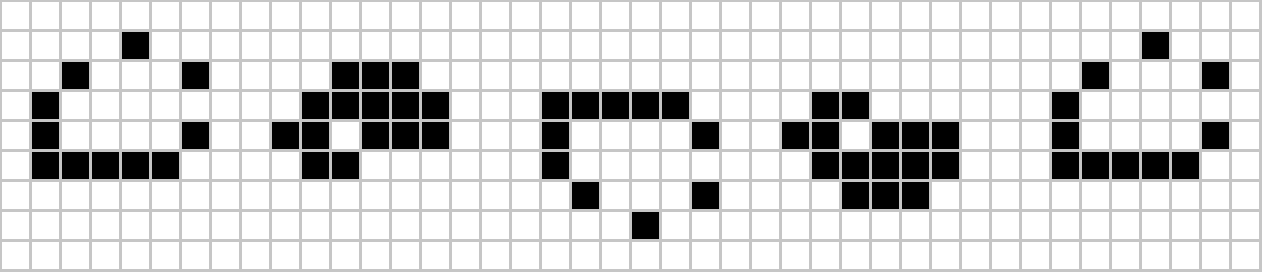
\includegraphics[width=\textwidth]{./images/middleweightspaceship_evo.png}
    \caption{De derecha a izquierda, evolución síncrona de la configuración \textit{middleweight spaceship}.}
    \label{fig:middleweightspaceship_evo}
\end{figure}

Al igual que en la configuración anterior, \textit{middleweight spaceship}, el número de clústeres permanece constante independientemente del valor de $\alpha$. Y tanto el promedio de nodos ocupados como el de densidad tienen el mismo comportamiento. Sin embargo para el valor medio de área se produce una variación del comportamiento que se puede observar en la \autoref{fig:88}. El área varía prácticamente de la misma manera para $\alpha=0.15, 0.75$ y a excepción de $\alpha=0.90$ el resto de valores de $\alpha$ muestran un comportamiento constante muy parecido entre sí a partir de la vigésima iteración. Algo que sí coincide con el comportamiento de la configuración anterior es que $\alpha=0.90$ es el promedio de área que más cercano de sitúa del valor obtenido en las iteraciones de la evolución síncrona. Otra diferencia notable es que la longitud del intervalo en el que varía el promedio crece aproximadamente una unidad.

La siguiente configuración que vamos a estudiar, \textit{heavyweight spaceship} muestra un aspecto similar a las dos anteriores tanto en forma como en su evolución síncrona. En la \autoref{fig:heavyweightspaceship_evo} se muestran 4 iteraciones de esta configuración inicial. Se trata de una configuración de velocidad $c/2$ que se desplaza paralelamente al eje horizontal con un área constante de 35 \textit{nodos}$^2$. En las iteraciones pares tiene 13 nodos ocupados agrupados en tres clústeres con un calor de [MISSING VALUE!] nodos y en las iteraciones impares tiene 18 nodos agrupados en un solo clúster con un calor de [MISSING VALUE!] nodos.

\begin{figure}[H]
	\centering
    \includegraphics[width=\textwidth]{./images/data/middleweightspaceship/{Area_multiple_alpha}.png}
    \caption{Variación del área media en la configuración \textit{middleweight spaceship} para distintos valores de $\alpha$.}
    \label{fig:88}
\end{figure}

\begin{figure}[H]
	\centering
    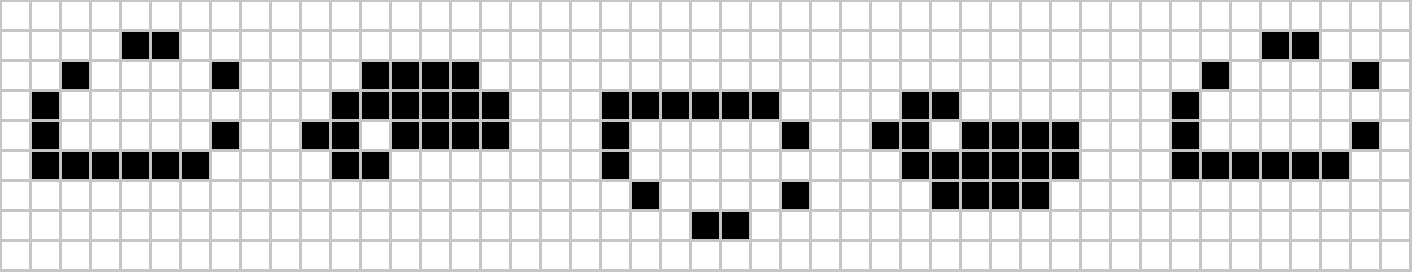
\includegraphics[width=\textwidth]{./images/heavyweightspaceship_evo.png}
    \caption{De derecha a izquierda, evolución síncrona de la configuración \textit{heavyweight spaceship}.}
    \label{fig:heavyweightspaceship_evo}
\end{figure}

A diferencia de las anteriores \textit{naves espaciales}, en la configuración \textit{heavyweight spaceship} el número de clústeres no se mantiene constante independientemente del valor que $\alpha$ tome. En la \autoref{fig:9-1} es posible observar este cambio, además todos los valores medios se mantienen aproximadamente constantes a partir de la décima iteración. A medida que $\alpha$ incrementa se visualiza que la separación vertical de los valores constantes del promedio de clústeres no es constante como en las \textit{naves espaciales} anteriores (\autoref{fig:7-2}) y dicha separación incrementa con el valor de $\alpha$.

Por otra parte, la densidad media también experimenta un comportamiento diferente en situación de $\alpha$-asincronismo en la evolución (\autoref{fig:9-2}). De nuevo a partir de la décima iteración los promedios se mantienen aproximadamente constantes pero ahora en lugar de decrecer con el crecimiento de $\alpha$, crecen de algo menos de 0.35 a algo más de 0.55 \textit{nodos}$^{-1}$.

El desarrollo en situación de $\alpha$-asincronismo que experimenta el valor medio de área es un comportamiento mucho más acentuado que los anteriores. Esto es, el intervalo en el que oscila el área media para distintos valores de $\alpha$ crece hasta una longitud de 8 \textit{nodos}$^{-1}$, siendo para $\alpha=0.9$ el menor valor de área, 31 \textit{nodos}$^2$ y para $\alpha=0.30, 0.45$ los mayores valores medios, aproximadamente 39 \textit{nodos}$^2$.

Los promedios de calor y número de nodos ocupados muestran un comportamiento idéntico al que se puede observar en la \autoref{fig:7-2}.

\begin{figure}[H]
	\centering
    \includegraphics[width=\textwidth]{./images/data/heavyweightspaceship/{Clusteres_multiple_alpha}.png}
    \caption{Variación del promedio de clústeres en la configuración \textit{heavyweight spaceship} para distintos valores de $\alpha$.}
    \label{fig:9-1}
\end{figure}

\begin{figure}[H] 
    \centering
    \includegraphics[width=\textwidth]{./images/data/heavyweightspaceship/{Densidad_multiple_alpha}.png}
    \caption{Variación del promedio de densidad en la configuración \textit{heavyweight spaceship} para distintos valores de $\alpha$.}
    \label{fig:9-2}
\end{figure}

Por último, la configuración inicial \textit{glider} es una nave espacial de velocidad $c/4$ formada por 5 nodos ocupados agrupados en un único clúster, tiene un calor de 4 \textit{nodos} y ocupa un área de 9 \textit{nodos}$^2$ (\autoref{fig:glider_evo}). Esta configuración inicial desarrolla un comportamiento sorprendentemente similar al descrito para los osciladores de periodo 2 en la sección \ref{osci2}.

\begin{figure}[H]
	\centering
    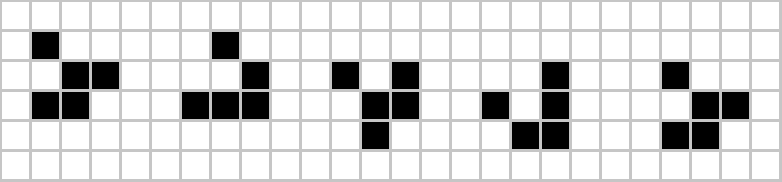
\includegraphics[width=\textwidth]{./images/glider_evo.png}
    \caption{Evolución síncrona de la configuración \textit{glider}.}
    \label{fig:lightweightspaceship_evo}
\end{figure}

% Existen dos intervalos bien marcados, uno de decrecimiento (que va disminuyendo en tamaño) y otro de crecimiento que va creciendo
%\section{Efecto de la variación de la distribución de probabilidad}

%En esta sección vamos a estudiar el efecto de la generación de números aleatorios para las simulaciones utilizando distribuciones de probabilidad distintas a la uniforme. Nos resulta de especial interés algún tipo de distribución que este relacionada con el valor de $\alpha$-asincronicidad que empleemos. Una buena candidata es la distribución normal con media $\mu=\alpha$

%Cuidado, una normal centrada el $\alpha$ no da valores entre 0 y 1, hay que hacer alguna magia más


\end{document}